\documentclass[12pt]{article}
%\setlength{\mathindent}{2cm}\setlength{\voffset}{0cm}
\setlength{\hoffset}{-1.85cm}\setlength{\textwidth}{17.75cm}
\setlength{\textheight}{23cm} \setlength{\topmargin}{-2.0cm}
\renewcommand{\baselinestretch}{1}
\usepackage{rotating}
\usepackage{color}
\usepackage{amssymb}
\usepackage{amsmath,amsthm}
\DeclareMathOperator{\sech}{sech}
\usepackage{amsfonts}
\usepackage{graphicx}
\usepackage{graphics}
\usepackage{setspace}
\usepackage{booktabs}
\usepackage{algorithm2e}
\numberwithin{equation}{section}
\newtheorem{Theorem}{Theorem}[section]
\newtheorem{Example}[Theorem]{Example}
\newtheorem{Proposition}[Theorem]{Proposition}
\newtheorem{Definition}[Theorem]{Definition}
\newtheorem{cor}{Corollary}
\newtheorem{lemma}[Theorem]{Lemma}
\newtheorem{ex}[Theorem]{Example}
\newtheorem{Remark}[Theorem]{Remark}
%\pagenumbering{arabic}
%----------------------------------------------------------
\begin{document}
\date{\small\textsl{\today}}
\title{Application of Direct Meshless Local Petrov-Galerkin (DMLPG) method for some Turing-type models}
%%%%%%%%%%%%%%%%%
\author{
 \large Mohammad Ilati, \large Mehdi Dehghan\footnote{Corresponding author.  {\em E-mail addresses:}\
m.ilati@aut.ac.ir (M. Ilati), mdehghan@aut.ac.ir, mdehghan.aut@gmail.com (M. Dehghan)
}   \,  $^{\mbox{\small \em }}$ \\
\small{\em $^{\mbox{\footnotesize }}$\em  Department of Applied Mathematics, Faculty of Mathematics and Computer Science,}\vspace{-1mm}\\
 \small{\em $^{\mbox{\footnotesize }}$\em  Amirkabir University of Technology, No. 424,
Hafez Ave., 15914, Tehran, Iran}\vspace{-1mm}\\
} \maketitle
%%%%%%%%%%%%%%%%%%
\vspace{.9cm} %\hline\\  \noindent\\ \abst\\ \\

\begin{abstract}
Mathematical modelling of pattern formation in developmental biology is caused to non-linear reaction-diffusion systems which are usually highly stiff in both diffusion and
reaction terms. In this paper, the
Direct Meshless Local Petrov-Galerkin (DMLPG) procedure is applied to find the
numerical solution of some non-linear time-dependent reaction-diffusion systems such as Schnakenberg model, Gierer-Meinhardt model, FitzHugh-Nagumo model and Gray-Scott model. As far as we know, it is the first time that DMLPG method is applied for solving non-linear partial differential equations (PDEs) and systems of PDEs. Computational efficiency is the most significant
advantage of the DMLPG method in comparison with the classic Meshless Local Petrov-Galerkin (MLPG) method. This is due to the fact that DMLPG shifts the numerical
integrations over low-degree polynomials instead of over complicated moving least squares (MLS) shape functions and this reduces the computational costs, significantly. The main aim of this paper is to show that the DMLPG method is also suitable for solving the non-linear time-dependent systems especially reaction-diffusion systems. Numerical results support the good efficiency of the proposed method for solving non-linear reaction-diffusion systems. Also it is shown that DMLPG provides considerable savings in computational time in comparison with the classical MLPG method.
\vspace{.5cm}\\
\textbf{Keywords}: Meshless local weak form methods, Generalized moving least squares (GMLS) approximation, MLPG methods, Direct MLPG (DMLPG) methods, Schnakenberg model, Gierer-Meinhardt model, FitzHugh-Nagumo model, Gray-Scott model.\\\\%\hline \\ \\
\textbf{AMS Subject Classifications}: 65M99; 65N99
\end{abstract}
%\newpage

\section{Introduction}
Mathematical modelling of problems in developmental biology
has caused to a variety of models which employed for spatial-temporal patterning phenomena.  Many of these mathematical models are reaction-diffusion systems~\cite{WazwazBook}.
At first, Turing in his seminal paper concerning morphogenesis \cite{Turing1}, planned a novel concept of diffusion driven instability in reaction-diffusion systems. After that, the reaction-diffusion theory of pattern formation has been widely
applied to different fields of sciences.\\
In general, the reaction-diffusion system has the following form
\begin{equation}\label{RDO}
\frac{{\partial {\mathbf{u}}}}{{\partial t}} = D{\nabla ^2}{\mathbf{u}} + R({\mathbf{u}}),\end{equation}
where ${\mathbf{u}}=[u,v]^T\in{\mathbb{R}}^{2}$
represents concentrations of a group of biochemical molecules,
  $D=diag\{d_1,d_2\}\in{\mathbb{R}}^{2\times 2}$
is the diffusion constant
matrix, ${\nabla ^2}{\mathbf{u}}$
is the Laplacian associated with the diffusion of the molecule whose concentration is ${\mathbf{u}}$, and $R({\mathbf{u}})$ describes the biochemical reactions.\\
Some well-known Turing-type models are the Gierer-Meinhardt model \cite{Gierer}, the Schnakenberg model \cite{Schnak}, the
Thomas model \cite{Thomas}, the Gray-Scott model \cite{Gray1,Gray2}, Lengyel-Epstein model \cite{Lengyel}, Brusselator model \cite{Prigogine}, FitzHugh-Nagumo model (FHN) \cite{Fitz1,Fitz2, Nagu} and Sel'klov model \cite{Selkov}.
\par
Basic theoretical aspects of the Turing problem have been investigated in considerable detail \cite{Borckmans, De, Walgraef} and it has been
illustrated in essence how biological patterns can arise from the Turing instability \cite{Murray}. Also, some numerical algorithms
have been employed to solve and analysis some Turing models:
Four cases have been analyzed and
have been solved numerically using finite element method in \cite{Garz}. Authors of \cite{Ilati} have proposed the meshless local weak form method based on a new combined shape function to find the numerical solution of time-dependent non-linear Brusselator and Gierer-Meinhardt systems.
In \cite{Tatari}, finite
point method (FPM)  has been developed for non-linear reaction-diffusion systems which are often
employed in mathematical modeling of developmental biology. Authors of \cite{Sladek} have proposed
a meshless local integral equation (LIE) method for computational simulation of 2D pattern
formation in non-linear reaction-diffusion systems. Authors of \cite{Shakeri} have developed a hybrid finite volume spectral element method for the numerical solution of Turing system generated by Schnakenberg model. In \cite{FitzNagu}, a numerical method for inverse problem of FitzHugh-Nagumo and Aliev-Panfilov models has been proposed, and the numerical results for regions similar to different sections of a heart have been presented. Authors of
\cite{Ambrosio} have studied synchronization and control analysis of reaction-diffusion FitzHugh-Nagumo type system. In \cite{Ruuth}, the performance of several of the best known linear multistep implicit-explicit (IMEX) schemes for solving reaction-diffusion problems in pattern formation has been analyzed. Authors of \cite{Arraras}, have applied the domain decomposition multigrid methods  for solving nonlinear reaction-diffusion problems.
In \cite{Zhu}, discontinuous Galerkin (DG) finite element methods, coupled with Strang type
symmetrical operator splitting methods, have been used for solving reaction-diffusion systems in
domains with complex geometry. The authors of \cite{Zhang} have presented numerical solutions of Schnakenberg model and chloride-iodide-malonic acid
(CIMA) reactive model, by combining direct discontinuous Galerkin (DDG) finite element method with implicit integration factor (IIF) time integration method. In \cite{Abbaszadeh2}, variational multiscale element free Galerkin (VMEFG) and local discontinuous Galerkin (LDG) methods have been applied for solving two-dimensional Brusselator reaction-diffusion system with and without cross-diffusion.


\subsection{A brief review of the DMLPG method}
In this paper, we propose DMLPG method for solving non-linear time-dependent reaction-diffusion systems in developmental biology.  It is well-known that, in the classical meshless local Petrov-Galerkin method
%\cite{Atluri, Atluri1, Atluri2, Dai1, Dai2,Dai3, Abbaszadeh,Ghesmati,Salehi2,Salehi, Dong, Mazzia1, Shirzadi, Shirzadi2,Shivanian, %Shivanian2,Shivanian3,Wang,Wei,ZhangT},
%%
\cite{Atluri, Atluri1, Atluri2, Dai1, Dai2,Dai3, Ghesmati,Salehi2,Salehi, Dong, Mazzia1, Shirzadi, Shirzadi2,Shivanian, Shivanian2,Shivanian3,Wang,Wei,ZhangT},
%%
the numerical integration of local weak form
over the moving least squares shape functions is computationally expensive. To overcome this shortage, direct meshless local Petrov-Galerkin (DMLPG) method was proposed by Mirzaei and Schaback \cite{Mirzaei}. In the DMLPG method, numerical integrations are done over low-degree polynomials instead of complex shape functions and this leads to much cheaper computational cost. In other words, in DMLPG, shape functions are ignored completely. This advantage is achieved using a generalized moving least squares approximation \cite{Mirzaei1}, where
a test functional is approximated in terms of nodes without applying shape functions. Altogether, the DMLPG method is simpler and faster than
original MLPG.
Similar to MLPG, DMLPG method solves PDEs in local weak form and integrations breaks down to some regular, well-shaped and
independent sub-domains. Therefore, no global background cell is required to
calculate integrals and thus the DMLPG is known as a truly meshless method.\\
Since DMLPG
significantly uses less computational time in comparison with the MLPG method, the DMLPG
method can be an attractive procedure for computer modeling and simulation of problems in engineering and applied sciences. For example, the authors of \cite{Mazzia} numerically analyzed the solution of 2D and 3D potential problems via DMLPG. In \cite{taleei}, DMLPG method is applied for solving elliptic interface problems. In \cite{Sartoretto}, the DMLPG technique is applied for 3D Poisson problems. The author of \cite{MirzaeiT}, developed DMLPG method for solving two and three dimensional problems in elasticity. In \cite{MirzaeiRamezani}, DMLPG method applied for
solving a two-dimensional time fractional advection-diffusion equation. An
application to elastodynamic analysis can be found in \cite{Mirzaei4}. Moreover, for the first time, in \cite{MirzaeiH} Mirzaei and Schaback applied DMLPG for solving time-dependent problems.

\subsection{The main aim of the current paper}
The main aim of this manuscript is to show that the DMLPG method is also suitable for solving the
system of non-linear PDEs especially reaction-diffusion systems. In this manuscript, we explain how one can apply the DMLPG method for solving non-linear time-dependent partial differential equations (PDEs) as well as systems of PDEs.  In addition, the DMLPG method is compared with the classic MLPG methods in terms of computational cost and better efficiency of DMLPG is shown.\par
The organization of the rest of the current manuscript is as follows: in Section 2, a brief
discussion about the generalized moving least squares approximation is outlined. A discritization process is described in Section 3. In Section 4, results of numerical experiments are
demonstrated. Finally Section 5 completes
the structure of this paper with a brief conclusion.

\section{Generalized moving least squares approximation}
The Moving Least Squares (MLS) method \cite{Abbaszadeh3,Lancaster,Li,Liew} was
proposed for approximating a function $u(\mathbf{x})$ inside a region $\Omega\subset \mathbb{R}^{d}$ using the values $u(\mathbf{x}_{j})$ at nodes $X=\{\mathbf{x}_{j}\}_{j=1}^{N}$. It should be noted that, for the sparsity of the final coefficient matrix, the set $X$ can be
replaced by a subset that consists only the nodes that are located on the neighbourhood of the point of interest.
In the context of MLPG methods, the MLS  is applied for approximating the unknown function $u$ on the ground of a suitable ``\ weight''
function \cite{Liu}. \\
Similar to most meshless methods, in the MLS approximation method, trial functions can be written as linear combinations of MLS shape functions ${\varphi _1},...,{\varphi _N}$ as
\begin{equation}
u(\mathbf{x}) = \sum\limits_{j = 1}^N {{\varphi _j}(\mathbf{x})u({\mathbf{x}_j})},\end{equation}
in terms of values at nodes.\\
Suppose that, after discretizing the PDE problem, the following equations are obtained
\begin{equation}\label{F1}
{\lambda _i}(u) = {\beta _i},\,\,\,\,\,\,\,\,\,\,\, i=1,...,M,
\end{equation}
where the functionals ${\lambda _1},...,{\lambda _M}$ can, for instance, describe point evaluations of $u$, its derivatives, or some local integrals over $u$ or its derivatives.\\ It's worth mentioning that, if these functionals are chosen to be the
point evaluations of $u$, then the classical MLS approximation is resulted.
Using the MLS approximation techniques, equations (\ref{F1}) are approximated as follows
\begin{equation}
{\lambda _i}(u) = \sum\limits_{j = 1}^N {{\lambda _i}({\varphi _j})u({\mathbf{x}_j})}  = {\beta _i},\,\,\,\,\,\,i=1,...,M.\end{equation}
It is obvious that, all functionals must be
specified on all shape functions, and this is a tiresome procedure
if the shape functions are not cheap to specify, and it is even more tiresome if the
functionals consist of integrations of derivatives against test functions \cite{MirzaeiH}.\\
For overcoming this drawback, the Generalized Moving Least Squares (GMLS) method \cite{Mirzaei1} was developed for approximating continuous linear functionals in the dual of $C^{r}(\Omega)$, for any $r\geq0$.
According to GMLS approximation technique, each
functional ${\lambda _i}$ can be well approximated in terms of nodal values by a formula
\begin{equation}\label{F2}
{\lambda _i}(u) = \sum\limits_{j = 1}^N {{\alpha _{ji}}u({\mathbf{x}_j})}.
\end{equation}
Therefore for obtaining unknown values, the following system is solved without any use of shape functions.
\begin{equation}
\sum\limits_{j = 1}^N {{\alpha _{ji}}u({\mathbf{x}_j})}  = {\beta _i},\,\,\,\,\,\,\,\,\,\,\,i=1,...,M.
\end{equation}
Efficient ways must be applied to the approximation (\ref{F2}). Here we employ a generalized version of Moving Least Squares (MLS) procedure, adapted from \cite{Mirzaei1}.\\
The techniques of \cite{Mirzaei1} and \cite{Mirzaei} allow to calculate coefficients ${{\alpha _{ji}}}$ for (\ref{F2}) very effectively as follows \cite{MirzaeiH}:\\
The aim is calculating a coefficient vector $a({\lambda _i}) = {({\alpha _{1i}},...,{\alpha _{Ni}})^T} \in \mathbb{R}^{N}$
for (\ref{F2}). A space $\mathcal{P}$ of polynomials is chosen which is large enough
to let zero be the only polynomial $p$ in $\mathcal{P}$ that vanishes on $X$. Consequently, the
dimension $m$ of $\mathcal{P}$ satisfies $m\leq N$, and the $m \times N$ matrix $P$ of values $p_{k}(\mathbf{x}_{j})$ of
a basis ${p_1},...,{p_m}$ of $\mathcal{P}$ has rank $m$. Therefore for any vector $w = {({w_1},...,{w_N})^T}$ of
positive weights, the generalized MLS solution $a({\lambda _k})$ to (\ref{F2}) can be written as \cite{MirzaeiH}
\begin{equation}\label{alambda}
a({\lambda _i}) = W{P^T}{(PW{P^T})^{ - 1}}{\lambda _i}(\mathcal{P}),
\end{equation}
where $W$ is the diagonal matrix with diagonal $w$ and
${\lambda _i}(\mathcal{P}) = {({\lambda _i}({p_1}),...,{\lambda _i}({p_m}))^T} \in \mathbb{R}^{m}$.\\
One can see, ${\lambda _i}$ acts only on polynomial basis functions and since the coefficient
matrix in (\ref{alambda}) is independent of $i$, the same matrix can be employed for different ${\lambda _i}$ as long
as $X$ does not change locally. As mentioned in \cite{MirzaeiH}, this will significantly speeds up numerical calculations,
if the functional ${\lambda _i}$ is complicated, e.g. a numerical integration against a test function \cite{MirzaeiH}. Note that the MLS shape functions are ignored completely. But the
weights will be specified locally in the same way as in the MLS.

\section{Discretization process}
In this section, at first, the temporal space is discretized using finite difference scheme. Then full discretization based on meshless local weak forms is obtained.\\
For the discretization of the time variable,
we need to set up some preliminary notation \[{t_k} = k\tau ,\,\,\,\,\,\,\,\,\,\,\,k = 0,1,2,...,M,\]
where $\tau  = {T \mathord{\left/
 {\vphantom {T M}} \right.
 \kern-\nulldelimiterspace} M}$ is the step size of time variable and $T$ is final time.\\ To deal with the time derivative, a time-stepping method based on famous Crank-Nicolson scheme is employed.
\begin{equation}\frac{{{\mathbf{u}^{k + 1}} - {\mathbf{u}^k}}}{\tau } = D\frac{{{\nabla ^2}{\mathbf{u}^{k + 1}} + {\nabla ^2}{\mathbf{u}^k}}}{2} + R({\mathbf{u}^k}).\end{equation}
The simplified form can be written as:
\begin{equation}\label{Gzaman}
{\mathbf{u}^{k + 1}} - \frac{\tau }{2}D{\nabla ^2}{\mathbf{u}^{k + 1}} = {\mathbf{u}^k} + \frac{\tau }{2}D{\nabla ^2}{\mathbf{u}^k} + \tau R({\mathbf{u}^k}).\end{equation}
For the space discretization, the weak forms are used to providing a set of algebraic equations. These algebraic equations are obtained by numerical integration over the domain of the problem, globally or locally. In the global weak-form case, the global integral form must be satisfied over the entire problem
domain, and hence, a set of background cells has to be used for the
numerical integration. Therefore these methods are not truly
meshless methods.  To avoid the use of global background cells, the so-called local weak-form methods have been developed. In local weak-form, the numerical
integrations are carried out over a local quadrature domain defined for the field
node. Therefore, no global background mesh is required \cite{Liu}.\\
Here, at first, the MLPG method is applied for space discretization. Then based on the MLPG formulation, the DMLPG method is introduced which is fast.\\
In the standard MLPG, around each $\mathbf{x}_i$ a small sub-domain $\Omega _i \subset \bar \Omega $
is chosen such that integrations over  $\Omega _i$ are comparatively cheap. The local sub-domains overlap each other, and cover the whole global domain $\Omega$. The local sub-domains could be of any geometric shape and size.  For simplicity they
are taken to be of circular shape. The local weak form of the approximate equations (\ref{Gzaman}) for $\mathbf{x}\in \Omega _i$
can be written as
\begin{equation}
\int\limits_{{\Omega _i}} {{\mathbf{u}^{k + 1}}\nu d\Omega }  - \frac{\tau }{2}D\int\limits_{{\Omega _i}} {{\nabla ^2}{\mathbf{u}^{k + 1}}\nu d\Omega }  = \int\limits_{{\Omega _i}} {{\mathbf{u}^k}\nu d\Omega }  + \frac{\tau }{2}D\int\limits_{{\Omega _i}} {{\nabla ^2}{\mathbf{u}^k}\nu d\Omega }  + \tau \int\limits_{{\Omega _i}} {R({\mathbf{u}^k})\nu d\Omega } ,\end{equation}
where $\nu$ is a test function. Using the divergence theorem we obtain
\begin{equation}\label{FDI}
\begin{array}{l}
\int\limits_{{\Omega _i}} {{\mathbf{u}^{k + 1}}\nu d\Omega }  - \frac{\tau }{2}D\Big[\int\limits_{{\partial \Omega _i}} {\nabla {\mathbf{u}^{k + 1}}.n\,\nu d\Omega }  - \int\limits_{{\Omega _i}} {\nabla {\mathbf{u}^{k + 1}}.\nabla \,\nu d\Omega } \Big] = \\\\
\int\limits_{{\Omega _i}} {{\mathbf{u}^k}\nu d\Omega }  + \frac{\tau }{2}D\Big[\int\limits_{{\partial \Omega _i}} {\nabla {\mathbf{u}^k}.n\,\nu d\Omega }  - \int\limits_{{\Omega _i}} {\nabla {\mathbf{u}^k}.\nabla \,\nu d\Omega } \Big] + \tau \int\limits_{{\Omega _i}} {R({\mathbf{u}^k})\nu d\Omega } .
\end{array}\end{equation}
For boundary point $\mathbf{x}_i$, $\partial \Omega _i$ is replaced by $L_i \cup \Gamma _i$, where $\Gamma _i$
is a part of the local boundary located on the global boundary
and $L_i$ is the other part of the local boundary over which no
boundary conditions are specified, i.e., $\Gamma _i = \Omega _{i} \cap \partial \Omega $ and $L_i = \partial \Omega _{i} - \Gamma _i$. By imposing the natural boundary conditions
\begin{equation}\int\limits_{{\Gamma _i}} {\nabla {\mathbf{u}^{k + 1}}.n\,\nu d\Omega }  = \int\limits_{{\Gamma _i}} {\nabla {\mathbf{u}^k}.n\,\nu d\Omega }  = 0,\end{equation}
the local weak form equations for boundary points are
\begin{equation}\label{FDB}
\begin{array}{l}
\int\limits_{{\Omega _i}} {{\mathbf{u}^{k + 1}}\nu d\Omega }  - \frac{\tau }{2}D\Big[\int\limits_{{L _i}} {\nabla {\mathbf{u}^{k + 1}}.n\,\nu d\Omega }  - \int\limits_{{\Omega _i}} {\nabla {\mathbf{u}^{k + 1}}.\nabla \,\nu d\Omega } \Big] = \\\\
\int\limits_{{\Omega _i}} {{\mathbf{u}^k}\nu d\Omega }  + \frac{\tau }{2}D\Big[\int\limits_{{L _i}} {\nabla {\mathbf{u}^k}.n\,\nu d\Omega }  - \int\limits_{{\Omega _i}} {\nabla {\mathbf{u}^k}.\nabla \,\nu d\Omega } \Big] + \tau \int\limits_{{\Omega _i}} {R({\mathbf{u}^k})\nu d\Omega } ,
\end{array}\end{equation}
Although, DMLPG employs the same local weak forms obtained from a MLPG
formulation, but it is mathematically different from standard MLPG because direct approximations for local weak forms are provided. In DMLPG, the local weak forms are considered as functionals, then these functionals are approximated using GMLS approximation procedure. Therefore by considering the local integrals in (\ref{FDI}) and (\ref{FDB}) as functionals and using the GMLS approximation for these functionals, we obtain the linear system
\begin{equation}\label{LLS}
A{U^{k + 1}} = B{U^k} + b.\end{equation}
As we have already mentioned, numerical integrations are done over low-degree polynomials only, and no shape function is needed at all. This reduces the cost of numerical integration in MLPG method significantly.\\
It should be noted, the integrals of non-linear terms are approximated using GMLS approximation and then the accuracy of these approximations becomes better by applying the predictor-corrector algorithm. A brief description of the predictor-corrector algorithm is as follows.
\begin{center}
\begin{algorithm}[H]
\SetAlgoLined

\textbf{Predictor-corrector algorithm}\\
 $switch:=1$\;
 Solve linear system (\ref{LLS}) and obtain ${U^{k + 1}}$
\;
 Let ${U^ * }:={U^{k+1}}$
\;
 \While{$switch\ge1$}{
 solve linear system (\ref{LLS}) as follows:\\
 $A{U^{k + 1,\dag }} = B{U^k} + N({U^{ * }});$\\
  \eIf{$\left\|
{U^{k + 1,\dag }}-
{U^{* }} \right\| \le \varepsilon $}{
   $switch:=-1$\;
   }{
   $
{U^ * }:=
{U^{k + 1,\dag}}$\;
  }
 }
Save $
{U^{k + 1,\dag }}$ as a solution in step $k+1$.
\end{algorithm}
\end{center}

\section{Numerical results}
Implementation is done using the basis polynomials
\[{\left\{ {\frac{{{{(\mathbf x - {\mathbf x_i})}^\alpha }}}{{{h^{\left| \alpha  \right|}}}}} \right\}_{0 \le \left| \alpha  \right| \le m}},\]
where $h$ is the mesh size (fill distance) of point set $X$ in $\Omega$, and $\alpha  = ({\alpha _1},...,{\alpha _d}) \in \mathbb N_0^d$
is a
multi-index, and $\left| \alpha  \right| = {\alpha _1} + \cdots + {\alpha _d}$, here $d = 2$ \cite{Mirzaei4}.\\
In numerical results, we employ the quartic spline weight function in (G)MLS approximation for both MLPG and DMLPG methods.
\[w(\mathbf{x},{\mathbf{x}_i}) = w({\delta _i}) = \left\{ \begin{array}{l}
1 - 6\delta _i^2 + 8\delta _i^3 - 3\delta _i^4,\,\,\,\,\,\,\,{\delta _i} \le 1,\\
0,\,\,\,\,\,\,\,\,\,\,\,\,\,\,\,\,\,\,\,\,\,\,\,\,\,\,\,\,\,\,\,\,\,\,\,\,\,\,\,\,\,\,\,\,\,\,\,\,\,\,\,\,\,{\delta _i} > 1,
\end{array} \right.\]
where ${\delta _i} = \frac{{\left\| {\mathbf{x} - {\mathbf{x}_i}} \right\|}}{{{r_s}}}$ and $r_s$ is the radius of the support of the weight function. As mentioned in  \cite{MirzaeiT, MirzaeiH}, the parameter $r _s$ should be large enough to ensure the regularity of the moment matrix $PW{P^T}$ in (G)MLS approximation \cite{MirzaeiT, MirzaeiH}. The size of the support $r_s$ depends on $h$ (mesh-size) and degree of polynomials in use \cite{MirzaeiT}. Then the support size $r_s$ is an
important issue in meshless methods. The accuracy and efficiency of the meshless methods depend on the
number of nodes in the local support domain. Therefore, a suitable
support domain should be chosen to ensure an efficient and accurate
approximation. As mentioned in \cite{Liu}, the radius of support domain is determined by $r_s=\alpha_{s}h$ where $\alpha_s$ is the dimensionless size of the support domain, and $h$  is the fill distance. The dimensionless size of the support domain $\alpha_s$ controls the actual
dimension of the support domain and it is usually determined by carrying out numerical
experiments for a class of benchmark problems. Generally, an $\alpha_s=2.0\sim3.0$ leads to good results for many problems \cite{Liu}. Similar to the support domain, the size of quadrature domain can be chosen arbitrarily. The size of a quadrature domain is determined by $r_q=\alpha_{q}h$ where $\alpha_q$ is the dimensionless size of the quadrature domain, and $h$  is the fill distance. In order to ensure the quadrature domain is large
enough but always located entirely inside the computational domain, the value of $\alpha_q$ must be in the range of $0<\alpha_q<1$.\\
In this section, all of the numerical solutions are obtained by means of DMLPG method. Furthermore, the CPU times used for construction of coefficient matrices $A$ and $B$ in MLPG and DMLPG methods, are compared. Since the time stepping stage is the same in both MLPG and DMLPG methods, only the CPU times allocated for construction of coefficient matrices are compared. These comparisons show that, DMLPG method is absolutely faster than
MLPG method.\\
All routines were written using well-known symbolic software MATLAB
and run on a Pentium 4 PC with 8
GB of Memory and a Core(TM) i7-2600K 3.40 GHz CPU.

\subsection{Schnakenberg model}
This model is one of the simplest reaction-diffusion systems. The Schnakenberg model \cite{Schnak} is given by (\ref{RDO}) with
\begin{equation}
R(\mathbf u) = \left[ \begin{array}{l}
\gamma (a - u + {u^2}v)\\
\gamma (b - {u^2}v)
\end{array} \right],\end{equation}
where $a$, $b$ and $\gamma$ are constants. The Schnakenberg system \cite{Schnak} has been used to model the spatial distribution of a morphogen, e.g., the distribution of calcium in the hairs of the whorl in Acetabularia \cite{Goodwin}.
\subsubsection{Example 1}
As a first test problem consider the Schnakenberg model on the unit square domain $\Omega  = [0,1] \times [0,1]$
 with homogenous Neumann boundary conditions \cite{Shakeri,Tatari}. Let the parameter values be $a = 0.1$, $b = 0.9$, $d_1=1$,
$d_2=8.6676$ and $\gamma = 230.82$. $(u_s, v_s) =(1, 0.9)$ be the
homogeneous steady state of this problem. Initial conditions are taken as small random perturbations around this steady state. In this example, the numerical solutions are obtained with $h=1/30$, $\tau=0.001$, $r_q=0.95\,h$ and $r_s=2.05\,h$. The time evolution of the concentration of activator $u$ is shown in Fig. 1. We can
observe that the initial random perturbation is amplified and spreads, leading to
formation of checkered pattern presented in Fig. 1.
\begin{figure}\label{T1sch1}
\begin{center}
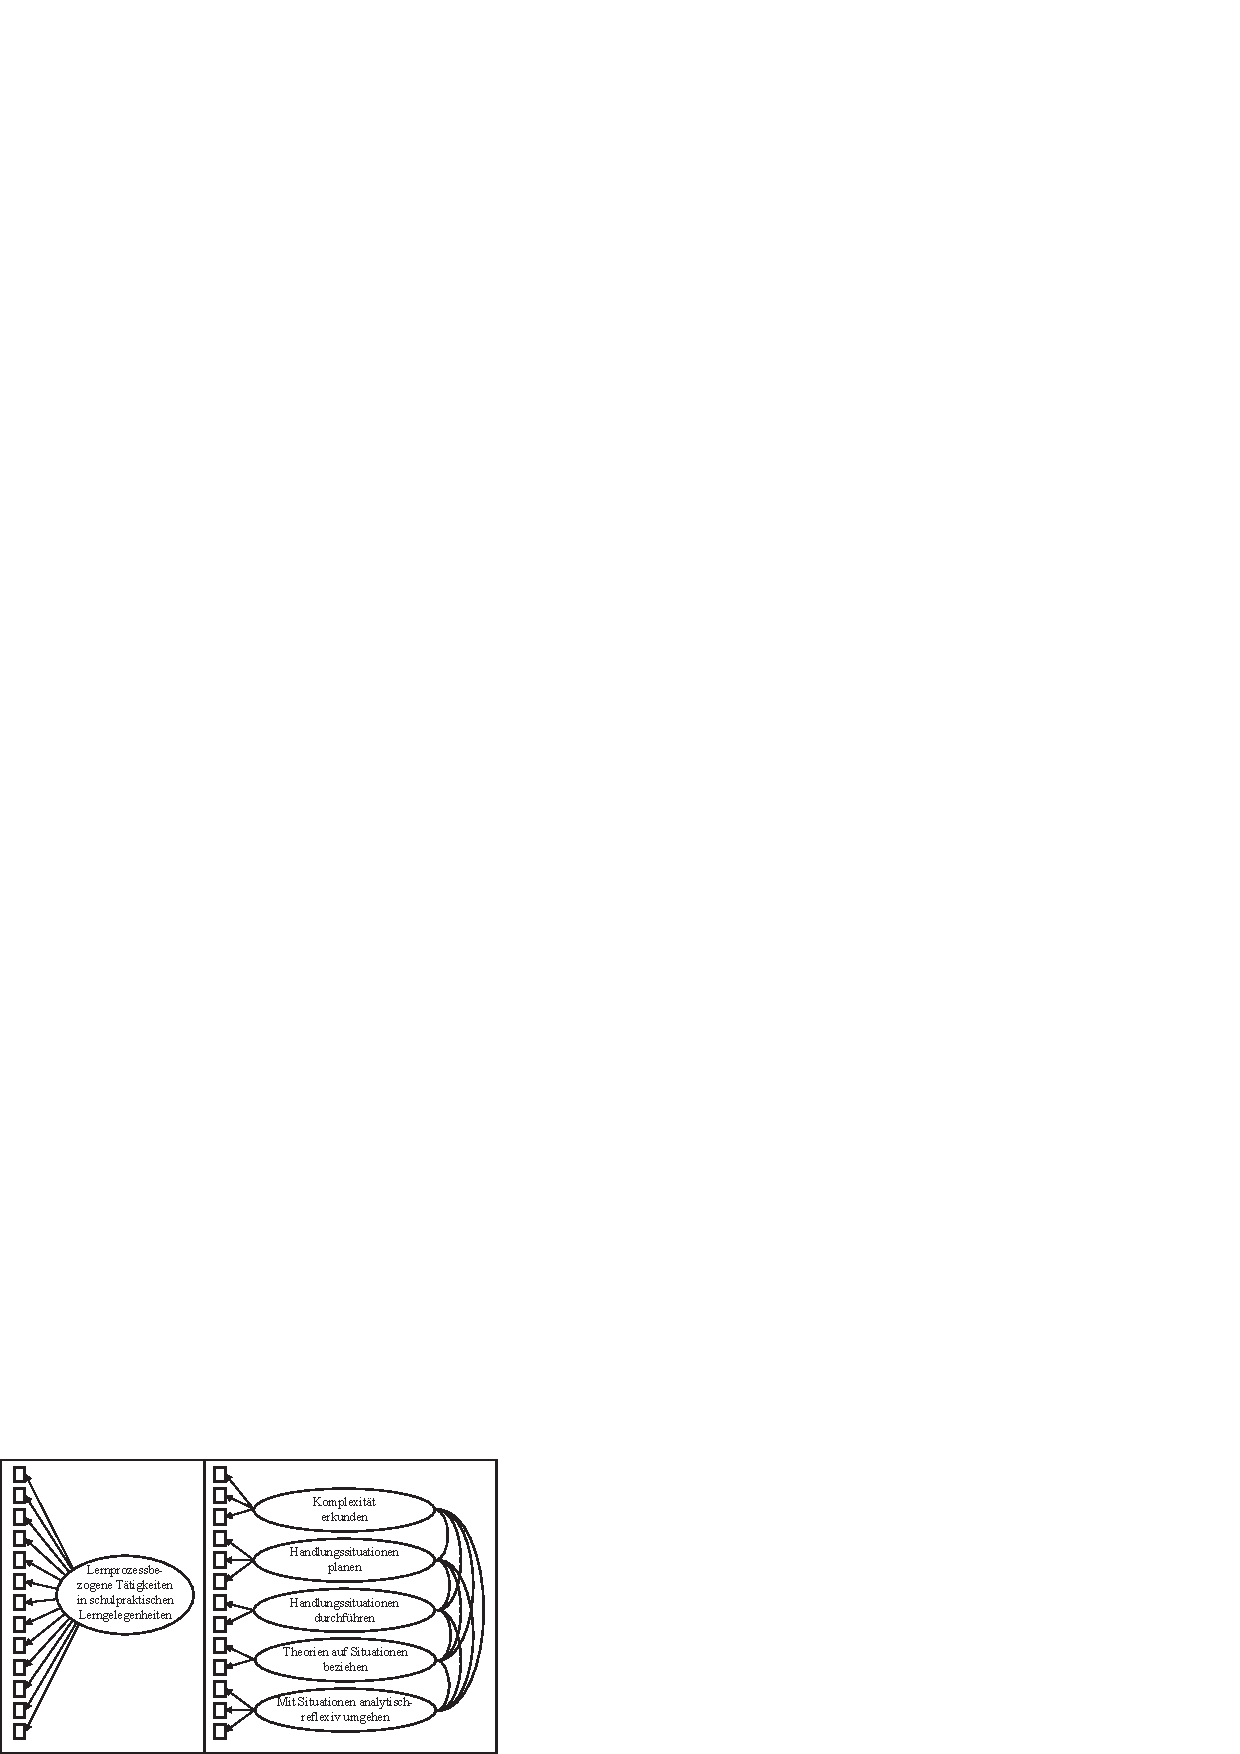
\includegraphics[width=8cm, height=7.cm]{Fig1.pdf}
\includegraphics[width=8cm, height=7.cm]{Fig2.pdf}
\includegraphics[width=8cm, height=7.cm]{Fig3.pdf}
\includegraphics[width=8cm, height=7.cm]{Fig4.pdf}
\includegraphics[width=8cm, height=7cm]{Fig5.pdf}
\includegraphics[width=8cm, height=7.cm]{Fig6.pdf}
\caption{Patterns generated by the Schnakenberg model with parameter values $a = 0.1$, $b = 0.9$, $d_1=1$,
$d_2=8.6676$ and $\gamma = 230.82$. Contour plots of time
evolution of the activator $u$ at different times. }
\end{center}
\end{figure}
Moreover, in Table 1 the CPU times allocated for construction of coefficient matrices in MLPG and DMLPG are
compared. As we can immediately see, DMLPG method is absolutely faster than
the classic MLPG method.
\begin {table}
\begin{center}
\begin{tabular}{cccr}
\multicolumn{4}{c} {{Table 1}}\\
\multicolumn{4}{c} {{Comparison of MLPG and DMLPG methods}}\\
\multicolumn{4}{c} {{in terms of CPU times used (Sec.)}}\\
\toprule
$h$       &&    DMLPG       &   MLPG  \\
\midrule
$\frac{1}{10}$  &&    $0.10$        &   $41.19$      \\
$\frac{1}{20}$  &&    $0.28$        &   $163.93$     \\
$\frac{1}{30}$  &&    $0.88$        &   $364.75$     \\
$\frac{1}{40}$  &&    $2.27$        &   $644.42$     \\
$\frac{1}{50}$  &&    $5.00$        &   $1003.57$    \\
\bottomrule
\end{tabular}
\end{center}
\end {table}
\subsubsection{Example 2}
Consider the Schnakenberg equations on the unit square domain $\Omega  = [0,1] \times [0,1]$ with homogenous Neumann boundary conditions applied to both $u$ and $v$ as before \cite{Zhang}. Let the parameter values determined by
$a = 0.1305$, $b = 0.7695$, $d_1=0.05$,
$d_2=1$ and $\gamma =100$. Initial conditions are considered as
\[\left\{ \begin{array}{l}
u(x,y,0) = a + b + {10^{ - 3}}{e^{ - 100\left( {{{(x - \frac{1}{3})}^2} + {{(y - \frac{1}{2})}^2}} \right)}},\\\\
v(x,y,0) = \frac{b}{{{{(a + b)}^2}}}.
\end{array} \right.\]
The numerical solutions are obtained with $h=1/30$, $\tau=0.0001$, $r_q=0.95\,h$ and $r_s=2.05\,h$. Fig. 2 shows the formation of spot patterns. In this figure, the concentration values of $u$ at different times are selected and illustrated.
\begin{figure}\label{T1sch2}
\begin{center}
\includegraphics[width=8cm, height=7.cm]{Fig7.pdf}
\includegraphics[width=8cm, height=7.cm]{Fig8.pdf}
\includegraphics[width=8cm, height=7.cm]{Fig9.pdf}
\includegraphics[width=8cm, height=7.cm]{Fig10.pdf}
\caption{Patterns generated by the Schnakenberg model with parameter values $a = 0.1305$, $b = 0.7695$, $d_1=0.05$,
$d_2=1$ and $\gamma = 100$. Contour plots of time
evolution of the activator $u$ at different times. }
\end{center}
\end{figure}
Moreover, in Table 2 the CPU times allocated for construction of coefficient matrices in MLPG and DMLPG techniques are
compared. As we can immediately see, DMLPG method is absolutely faster than
MLPG method.
\begin {table}
\begin{center}
\begin{tabular}{cccr}
\multicolumn{4}{c} {{Table 2}}\\
\multicolumn{4}{c} {{Comparison of MLPG and DMLPG methods}}\\
\multicolumn{4}{c} {{in terms of CPU times used (Sec.)}}\\
\toprule
$h$       &&    DMLPG       &   MLPG  \\
\midrule
$\frac{1}{10}$  &&    $0.10$        &   $41.03$      \\
$\frac{1}{20}$  &&    $0.29$        &   $161.90$     \\
$\frac{1}{30}$  &&    $0.89$        &   $363.43$     \\
$\frac{1}{40}$  &&    $2.22$        &   $659.96$     \\
$\frac{1}{50}$  &&    $4.89$        &   $1012.36$    \\
\bottomrule
\end{tabular}
\end{center}
\end {table}

\subsubsection{Example 3}
Consider the Schnakenberg equations on the unit square domain $\Omega  = [0,1] \times [0,1]$ with homogenous Neumann boundary conditions applied to both $u$ and $v$ \cite{Fernandes, Ruuth}. Let the parameter values be given by
$a = 0.126779$, $b = 0.792366$, $d_1=1$,
$d_2=10$ and $\gamma =1000$. Initial conditions are considered as
\[\left\{ \begin{array}{l}
u(x,y,0) = 0.919145 + 0.0016\cos (2\pi (x + y)) + 0.01\sum\limits_{j = 1}^8 {\cos (2\pi jx)} ,\\
v(x,y,0) = 0.937903 + 0.0016\cos (2\pi (x + y)) + 0.01\sum\limits_{j = 1}^8 {\cos (2\pi jx)} .
\end{array} \right.\]
The numerical solutions are obtained with $h=1/30$, $\tau=0.0001$, $r_q=0.95\,h$ and $r_s=2.05\,h$. Figures 3 and 4 show the concentration values of $u$ at different times.
\begin{figure}
\begin{center}
\includegraphics[width=8cm, height=7.cm]{Fig11.pdf}
\includegraphics[width=8cm, height=7.cm]{Fig12.pdf}
\includegraphics[width=8cm, height=7.cm]{Fig13.pdf}
\includegraphics[width=8cm, height=7.cm]{Fig14.pdf}
\includegraphics[width=8cm, height=7.cm]{Fig15.pdf}
\includegraphics[width=8cm, height=7.cm]{Fig16.pdf}
\caption{Patterns generated by the Schnakenberg model with parameter values $a = 0.126779$, $b = 0.792366$, $d_1=1$,
$d_2=10$ and $\gamma = 1000$. Time
evolution of the activator $u$ at different times. }
\end{center}
\end{figure}

\begin{figure}
\begin{center}
\includegraphics[width=8cm, height=7.cm]{Fig17.pdf}
\includegraphics[width=8cm, height=7.cm]{Fig18.pdf}
\includegraphics[width=8cm, height=7.cm]{Fig19.pdf}
\includegraphics[width=8cm, height=7.cm]{Fig20.pdf}
\includegraphics[width=8cm, height=7.cm]{Fig21.pdf}
\includegraphics[width=8cm, height=7.cm]{Fig22.pdf}
\caption{Patterns generated by the Schnakenberg model with parameter values $a = 0.126779$, $b = 0.792366$, $d_1=1$,
$d_2=10$ and $\gamma = 1000$. Contour plots of time
evolution of the activator $u$ at different times. }
\end{center}
\end{figure}

\subsubsection{Example 4}
In this example, we consider the Schnakenberg equations with parameter values
$a =-0.887757$, $b = 2.774242$, $d_1=1$,
$d_2=10$ and $\gamma =10000$ and compute solutions to the model equations on a unit square domain with homogenous Neumann boundary conditions applied to both $u$ and $v$ \cite{Fernandes}. Initial conditions are
taken as
\[\left\{ \begin{array}{l}
u(x,y,0) = 1.886485 + 0.001\sum\limits_{j = 1}^{37} {\frac{{\cos (2\pi jx)}}{j}} ,\\
v(x,y,0) = 0.779539 + 0.001\sum\limits_{j = 1}^{37} {\frac{{\cos (2\pi jx)}}{j}} .
\end{array} \right.\]
The numerical solutions are obtained with $h=1/30$, $\tau=0.00001$, $r_q=0.95\,h$ and $r_s=2.05\,h$.
The time evolution of the concentration of activator $u$ is shown in Figures 5 and 6.
\begin{figure}
\begin{center}
\includegraphics[width=8cm, height=7.cm]{Fig23.pdf}
\includegraphics[width=8cm, height=7.cm]{Fig24.pdf}
\includegraphics[width=8cm, height=7.cm]{Fig25.pdf}
\includegraphics[width=8cm, height=7.cm]{Fig26.pdf}
\includegraphics[width=8cm, height=7.cm]{Fig27.pdf}
\includegraphics[width=8cm, height=7.cm]{Fig28.pdf}
\caption{Patterns generated by the Schnakenberg model with parameter values $a = -0.887757$, $b = 2.774242$, $d_1=1$,
$d_2=10$ and $\gamma = 10000$. Time
evolution of the activator $u$ at different times. }
\end{center}
\end{figure}

\begin{figure}
\begin{center}
\includegraphics[width=8cm, height=7.cm]{Fig29.pdf}
\includegraphics[width=8cm, height=7.cm]{Fig30.pdf}
\includegraphics[width=8cm, height=7.cm]{Fig31.pdf}
\includegraphics[width=8cm, height=7.cm]{Fig32.pdf}
\includegraphics[width=8cm, height=7.cm]{Fig33.pdf}
\includegraphics[width=8cm, height=7.cm]{Fig34.pdf}
\caption{Patterns generated by the Schnakenberg model with parameter values $a = -0.887757$, $b = 2.774242$, $d_1=1$,
$d_2=10$ and $\gamma = 10000$. Contour plots of time
evolution of the activator $u$ at different times. }
\end{center}
\end{figure}

\subsection{Gierer-Meinhardt model}
The Gierer-Meinhardt model \cite{Gierer} comprises (\ref{RDO}) with
\begin{equation}
R(\mathbf u) = \left[ \begin{array}{l}
\gamma (a - bu + \frac{{{u^2}}}{{v(1 + K{u^2})}})\\
\gamma ({u^2} - v)
\end{array} \right],\end{equation}
where $a$, $b$ and $\gamma$ are positive parameters and $K$ is a measure of the saturation concentration.
As mentioned in \cite{Ghergu}, the model introduced by Gierer and Meinhardt has been
used with satisfactory quantitative results for modelling the head regeneration process
of hydra, an animal of few millimeters in length, consisting of 100,000 cells of about 15
different types and having a polar structure \cite{Ghergu}.

\subsubsection{Example 5}
In this example we solve the Gierer-Meinhardt reaction kinetics on the unit square domain $\Omega  = [0,1] \times [0,1]$ with homogenous
Neumann boundary conditions for both $u$ and $v$ \cite{Tatari}. Initial conditions are
taken as random perturbations about a constant value. Let the parameter values be given by
$a = 0.1$, $b =1$, $d_1=1$,
$d_2=70.8473$, $K=0.5$ and $\gamma =619.45$.
In this example, the numerical solutions are obtained with $h=1/20$, $\tau=0.001$, $r_q=0.75\,h$ and $r_s=2.15\,h$. The time evolution of the concentration of activator $u$ at different times is shown in Fig. 7.
\begin{figure}\label{FGM}
\begin{center}
\includegraphics[width=8cm, height=7.cm]{Fig35.pdf}
\includegraphics[width=8cm, height=7.cm]{Fig36.pdf}
\includegraphics[width=8cm, height=7.cm]{Fig37.pdf}
\includegraphics[width=8cm, height=7.cm]{Fig38.pdf}
\includegraphics[width=8cm, height=7.cm]{Fig39.pdf}
\includegraphics[width=8cm, height=7.cm]{Fig40.pdf}
\caption{Patterns generated by the Gierer-Meinhardt model with parameter values $a = 0.1$, $b = 1$, $d_1=1$,
$d_2=70.8473$, $K=0.5$ and $\gamma = 619.45$. Contour plots of time
evolution of the activator $u$ at different times. }
\end{center}
\end{figure}
In addition, in Table 3 the CPU times allocated for construction of coefficient matrices in MLPG and DMLPG techniques are
compared. As we can immediately see, DMLPG method is absolutely faster than
MLPG method.
\begin {table}
\begin{center}
\begin{tabular}{cccr}
\multicolumn{4}{c} {{Table 3}}\\
\multicolumn{4}{c} {{Comparison of MLPG and DMLPG methods}}\\
\multicolumn{4}{c} {{in terms of CPU times used (Sec.)}}\\
\toprule
$h$       &&    DMLPG       &   MLPG  \\
\midrule
$\frac{1}{10}$  &&    $0.11$        &   $42.71$      \\
$\frac{1}{20}$  &&    $0.29$        &   $171.21$     \\
$\frac{1}{30}$  &&    $0.91$        &   $385.80$     \\
$\frac{1}{40}$  &&    $2.38$        &   $692.72$     \\
$\frac{1}{50}$  &&    $5.32$        &   $1074.92$    \\
\bottomrule
\end{tabular}
\end{center}
\end {table}

\subsection{FitzHugh-Nagumo model}
The FitzHugh-Nagumo model (FHN) \cite{Fitz1,Fitz2, Nagu} is given by (\ref{RDO}) with
\begin{equation}
R(\mathbf u) = \left[ \begin{array}{l}
u (a - u )(u-1)-v\\
b u - \gamma v
\end{array} \right],\end{equation}
where $a$, $b$ and $\gamma$ are specified positive constants. The function $u$ is the transmembrane potential, and $v$ is a
slow restoring variable associated with ion currents \cite{Fitz1,Fitz2, Nagu}. As mentioned in \cite{FitzNagu, Sund}, this system describes the propagation of
excitation in the myocardium quite well. The FitzHugh-Nagumo model is used for analyzing various processes in the
myocardium. The electric activity of the heart has been simulated on its basis, including cases of the origination and propagation of helical waves \cite{Elkin,Medved}.

\subsubsection{Example 6}
In this example, we consider the FitzHugh-Nagumo model on domain $\Omega  = [-100,100] \times [-100,100]$ with homogenous Neumann boundary conditions for both $u$ and $v$ \cite{FitzNagu}. Let the parameter values be given by
$a = 0.15$, $b = 0.005$, $d_1=1$, and $\gamma =0.025$. Initial conditions are considered as
\[\left\{ {\begin{array}{*{20}{l}}
{u(x,y,0) = {e^{ - \left( {\frac{{{{(x - 30)}^2} + {y^2}}}{{16}}} \right)}},}\\
{}\\
{v(x,y,0) = 0.}
\end{array}} \right.\]
In this example, the numerical solutions are obtained with $h=4$, $\tau=0.04$, $r_q=0.75\,h$ and $r_s=2.15\,h$.
Figure 8 shows plots of the function $u$ at different times. A careful look at this figure shows the excitation is formed, how it propagates in the form of a wave, and how it passes through the boundary of the domain.
\begin{figure}\label{FHNF}
\begin{center}
\includegraphics[width=8cm, height=7.cm]{Fig41.pdf}
\includegraphics[width=8cm, height=7.cm]{Fig42.pdf}
\includegraphics[width=8cm, height=7.cm]{Fig43.pdf}
\includegraphics[width=8cm, height=7.cm]{Fig44.pdf}
\includegraphics[width=8cm, height=7.cm]{Fig45.pdf}
\includegraphics[width=8cm, height=7.cm]{Fig46.pdf}
\caption{Patterns generated by the FitzHugh-Nagumo model with parameter values $a = 0.15$, $b = 0.005$, $d_1=1$ and $\gamma = 0.025$. Plots of time
evolution of $u$ at different times. }
\end{center}
\end{figure}
\subsection{Gray-Scott model}
The Gray-Scott model \cite{Fernandes, ZhangK} is given by (\ref{RDO}) with
\begin{equation}
R(\mathbf u) = \left[ \begin{array}{l}
\gamma (1- u )- u{v^2}\\
u{v^2}-(\gamma+\kappa)v
\end{array} \right],\end{equation}
where $\gamma$
is the dimensionless flow rate (the inverse of the residence time) and $\kappa$ is decay constant of the activator, $v$.

\subsubsection{Example 7}
As the last example, we consider the two-dimensional Gray-Scott model with homogenous Neumann boundary conditions for both $u$ and $v$. We take the square domain $\Omega  = [-1,1] \times [-1,1]$. Let the parameter values be given by
$\gamma =1$, $\kappa =0$, $d_1=0.001$ and $d_2=0.001$. The exact solutions are considered as \cite{Fernandes, ZhangK}
\[\left\{ {\begin{array}{*{20}{l}}
{u(x,y,t) = \cos (2t)\cos (2\pi x)\cos (\pi y),}\\
{}\\
{v(x,y,t) = \cos (2t)\cos (\pi x)\cos (2\pi y).}
\end{array}} \right.\]
It is important to mention that Gray-Scott system has no explicit closed form solutions because of the non-linear reaction
terms. In order to measure the error norms, we first substituted the above-mentioned exact solutions into Gray-Scott system, and then
obtained the time-dependent source terms.
In this example, the numerical solutions are obtained with  $\tau=0.0001$, $r_q=0.75\,h$ and $r_s=2.15\,h$. This system is solved with both MLPG and DMLPG methods and
the maximum error norm ${L_\infty }$ for the components $u$ and $v$ with various values
of $h$ is shown in Table 4.
%As comes from
It can be observed via
%
Table 4, the DMLPG method gives better results for non-linear problems   compared with MLPG method. Moreover, in Table 5 the CPU times allocated for construction of coefficient matrices in MLPG and DMLPG methods are
compared. As we can immediately see, DMLPG method is absolutely faster than
the MLPG method.
Figures 9 and 10 show plots of the function $u$ and $v$ at $T=1$ computed by DMLPG method with $h=\frac{2}{{40}}$.
\begin {table}
\begin{center}
\begin{tabular}{ccccccccc}
\multicolumn{9}{c} {{Table 4: ${L_\infty }$ errors for
different values of $h$}}\\
\toprule
\multicolumn{2}{c}{} & \multicolumn{3}{c}{DMLPG}& \multicolumn{1}{c}{}& \multicolumn{3}{c}{MLPG}\\
\cmidrule(r){3-5}
\cmidrule(r){7-9}
$h$ && $L_\infty ^u$  &&  $L_\infty ^v$  & &$L_\infty ^u$ && $L_\infty ^v$ \\
\midrule
$\frac{2}{{10}}$ && $1.0041\times 10^{-3}$ && $1.9763 \times 10^{-3}$ && $2.7105\times 10^{-3}$&& $2.8649\times 10^{-3}$\\
$\frac{2}{{20}}$ && $4.1125\times 10^{-4}$ && $7.5140 \times 10^{-4}$ && $9.7185\times 10^{-4}$&& $1.5217\times 10^{-3}$\\
$\frac{2}{{30}}$ && $2.3619\times 10^{-4}$ && $3.5870 \times 10^{-4}$ && $3.6759\times 10^{-4}$&& $6.2657\times 10^{-4}$\\
$\frac{2}{{40}}$ && $1.7941\times 10^{-4}$ && $2.1702 \times 10^{-4}$ && $2.6969\times 10^{-4}$&& $3.4889\times 10^{-4}$\\
\bottomrule
\end{tabular}
\end{center}
\end {table}
\begin {table}
\begin{center}
\begin{tabular}{cccr}
\multicolumn{4}{c} {{Table 5}}\\
\multicolumn{4}{c} {{Comparison of MLPG and DMLPG methods}}\\
\multicolumn{4}{c} {{in terms of CPU times used (Sec.)}}\\
\toprule
$h$       &&    DMLPG       &   MLPG  \\
\midrule
$\frac{2}{10}$  &&    $0.11$        &   $41.21$      \\
$\frac{2}{20}$  &&    $0.30$        &   $161.59$     \\
$\frac{2}{30}$  &&    $0.89$        &   $380.74$     \\
$\frac{2}{40}$  &&    $2.27$        &   $649.28$     \\
\bottomrule
\end{tabular}
\end{center}
\end {table}
\begin{figure}
\begin{center}
\includegraphics[width=8cm, height=7.cm]{Fig47.pdf}
\includegraphics[width=8cm, height=7.cm]{Fig48.pdf}
\caption{Patterns generated by the Gray-Scott model with parameter values $\gamma = 1$, $\kappa = 0$, $d_1=0.001$ and $d_2=0.001$. Plots of time
evolution of $u$ and $v$ at $T=1$. }
\end{center}
\end{figure}
\begin{figure}
\begin{center}
\includegraphics[width=8cm, height=7.cm]{Fig49.pdf}
\includegraphics[width=8cm, height=7.cm]{Fig50.pdf}
\caption{Patterns generated by the Gray-Scott model with parameter values $\gamma = 1$, $\kappa = 0$, $d_1=0.001$ and $d_2=0.001$. Contour plots of time
evolution of $u$ and $v$ at $T=1$. }
\end{center}
\end{figure}

\section{Conclusions}
In this paper, we have applied DMLPG method for solving the two-dimensional non-linear time-dependent reaction-diffusion systems. In addition, we have compared DMLPG and MLPG procedures in terms of computational efficiency. Since local integrations are done over polynomials instead of over complicated MLS shape functions, the DMLPG method is considerably faster than the standard MLPG method. To show the accuracy and efficiency of the proposed method, some test problems have been investigated for reaction-diffusion systems of different types. Finally, we strongly believe that the DMLPG method has great potential to be replaced with the classic MLPG method in many situations.

{\bf Acknowledgement}:
%\section{Acknowledgement}
%\begin{quotation}
The authors thank both reviewers for their useful comments and
suggestions that improved the paper.
%\end{quotation}

\begin{thebibliography}{99}

\bibitem{Ambrosio} B. Ambrosio, M. A. Aziz-Alaoui, Synchronization and control of coupled reaction-diffusion
systems of the FitzHugh-Nagumo type, Comput. Math. Appl. 64 (2012) 934-943.

\bibitem{Arraras} A. Arraras, F. J. Gaspar, L. Portero, C. Rodrigo, Domain decomposition multigrid methods for
nonlinear reaction-diffusion problems, Commun. Nonlinear Sci. Numer. Simul.  20 (2015) 699-710.

\bibitem{Atluri} S. N. Atluri, The Meshless Method (MLPG) for Domain and BIE Discretizations, Tech Science Press, 2004.

\bibitem{Atluri1} S. N. Atluri, S. P. Shen, The meshless local Petrov-Galerkin (MLPG)method: A simple and less-costly alternative to the finite element methods, Computer Modeling in Engineering and Sciences (CMES) 3 (1) (2002) 11-51.

\bibitem{Atluri2} S. N. Atluri, T. Zhu,  A new meshless local Petrov-Galerkin (MLPG)
approach in computational mechanics, Comput. Mech. 22 (1998)
117-127.

\bibitem{Borckmans} P. Borckmans, A. De Wit, G. Dewel, Competition in ramped Turing structures, Physica A 188 (1992) 137-157.

\bibitem{Dai1} B. Dai, B. Zheng, Q. Liang, L. Wang,  Numerical solution of transient heat conduction problems using improved meshless local Petrov-Galerkin method, Appl. Math. Comput. 219 (2013) 10044-10052.

\bibitem{Dai2} B. Dai, J. Cheng, B. Zheng, A moving Kriging interpolation-based meshless local Petrov-Galerkin method for elastodynamic analysis, International Journal of Applied Mechanics 5 (2013) 1350011-21.

\bibitem{Dai3} B. Dai, Q. Wang, W. Zhang, L. Wang, The complex variable meshless local Petrov-Galerkin method for elastodynamic problems, Appl. Math. Comput. 243 (2014) 311-321.

\bibitem{Abbaszadeh2} M. Dehghan, M. Abbaszadeh, Variational multiscale element free Galerkin (VMEFG) and local discontinuous Galerkin (LDG) methods for solving two-dimensional Brusselator reaction-diffusion system with and without cross-diffusion, Comput. Methods in Appl. Mech. Eng. 300 (2016) 770-797.

%\bibitem{Abbaszadeh} M. Dehghan, M. Abbaszadeh, A. Mohebbi, Numerical solution of system of n-coupled nonlinear Schr\"{o}dinger equations via two %variants of the meshless local Petrov-Galerkin (MLPG) method, Computer Modeling Engineering and Sciences (CMES) 100 (2014) 399--444.

\bibitem{Abbaszadeh3} M. Dehghana, M. Abbaszadeh, A. Mohebbi, The numerical solution of the two-dimensional sinh-Gordon equation via three
meshless methods, Eng. Anal. Bound. Elem. 51 (2015) 220-235.

%_\bibitem{AbbaszadehEABE16}M. Dehghan, M. Abbaszadeh, A. Mohebbi, The use of element free Galerkin method based on moving Kriging and radial
%_ point interpolation techniques for solving some types of Turing models, Engineering Analysis with Boundary Elements, 62, (2016) 93--111 .

\bibitem{Ghesmati} M. Dehghan, A. Ghesmati, Numerical simulation of two-dimensional sine-Gordon solitons via a local weak meshless technique based 
on the radial point interpolation method (RPIM), Comput. Phys. Commun. 181 (2010) 772-786.

\bibitem{Salehi2} M. Dehghan, R. Salehi, A meshfree weak-strong (MWS) form method for the unsteady magnetohydrodynamic (MHD) flow in pipe with arbitrary wall conductivity, Comput. Mech. 52 (2013) 1445-1462.

\bibitem{Salehi} M. Dehghan, R. Salehi, A meshless local Petrov-Galerkin method for the time-dependent Maxwell equations, J. Comput. Appl. Math.  
268 (2014) 93-110.

\bibitem{De} A. De Wit, G. Dewel, P. Borckmans, D. Walgraef, Three-dimensional dissipative structures in reaction-diffusion systems, 
Physica D 61 (1992) 289-296.

\bibitem{Dong} L. Dong, A. Alotaibi, S. A. Mohiuddine, S. N. Atluri, Computational methods in engineering: a variety of primal and mixed methods, with global and local interpolations, for well-posed or ill-Posed BCs,  Computer Modeling in Engineering and Sciences (CMES) 99 (2014) 1-85.

\bibitem{Elkin} Yu. E. El'kin, A. V. Moskalenko, Ch. F. Starmer, Spontaneous halt of spiral wave drift in homogeneous excitable media, Mat. Biolog. Bioinform. 2(1) (2007) 73-81.

\bibitem{Fernandes} R. I. Fernandes, G. Fairweather,  An ADI extrapolated Crank-Nicolson orthogonal spline collocation
method for nonlinear reaction-diffusion systems, J. Comput. Phys. 231 (2012) 6248-6267.

\bibitem{Fitz1} R. FitzHugh, Mathematical models of threshold phenomena in the nerve membrane, Bull. Math. Biophys.
17 (1955) 257-278.

\bibitem{Fitz2} R. FitzHugh, Impulses and Physiological States in Theoretical Models of Nerve Membrane, Biophys. J. 1 (1961)
445-466.

\bibitem{Garz} D. A. Garzon-Alvarado, C. H. Galeano, J. M. Mantilla, Turing pattern formation for reaction-convection-diffusion systems in fixed domains submitted to toroidal velocity fields, Appl. Math. Model. 35 (2011) 4913-4925.

\bibitem{Ghergu} M. Ghergu, Steady-state solutions for Gierer-Meinhardt type systems with Dirichlet boundary
condition, Trans. Amer. Math. Soc. 361 (2009) 3953-3976.

\bibitem{Gierer} A. Gierer, H. Meinhardt, A theory of biological pattern formation, Kybernetik 12 (1972) 30-39.

\bibitem{Goodwin}  B. C. Goodwin, L. E. H. Trainor, Tip and whorl morphogenesis in Acetabularia by calcium-regulated strain fields, J. Theor. Biol. 117 (1985) 79-106.

\bibitem{Gray1} P. Gray,  S. K. Scott,  Autocatalytic reactions in the isothermal, continuous stirred tank reactor: isolas and
other forms of multistability, Chem. Eng. Sci. 38 (1) (1983) 29-43.

\bibitem{Gray2}  P. Gray,  S. K. Scott, Autocatalytic reactions in the isothermal, continuous stirred tank reactor: oscillations and the instabilities in the system $A+2B\rightarrow3B$, $B\rightarrow X$, Chem. Eng. Sci. 39 (6) (1984) 1087-1097.

\bibitem{Ilati} M. Ilati, M. Dehghan, Meshless local weak form method based on a combined basis function for numerical investigation of Brusselator model and spike dynamics in the Gierer-Meinhardt system, Computer Modeling in Engineering and Sciences (CMES), 109 (4) (2015) 325-360.

\bibitem{Lancaster}  P. Lancaster, K. Salkauskas, Surfaces generated by moving least
squares methods, Math. Comp. 37  (1981) 141-158.

\bibitem{Lengyel} I. Lengyel, I. R. Epstein, Modeling of Turing structures in the chlorite-iodidemalonic acid-starch reaction system, Science 251 (1991) 650-652.

\bibitem{Li} D. M. Li, F. N. Bai, Y. M. Cheng, K. M. Liew, A novel complex variable element-free Galerkin method for two-dimensional large deformation problems, Comp. Meth. Appl. Mech. Eng. 233-236 (2012) 1-10.

\bibitem{Liew} K. M. Liew, C. Feng, Y. M. Cheng, S. Kitipornchai, Complex variable moving least-squares method: a meshless approximation technique, Int. J. Numer. Meth. Eng. 70 (2007) 46-70.

\bibitem{Liu} G. R. Liu, Y. T. Gu, An Introduction to Meshfree Methods and Their Programming, Berlin: Springer, 2005.

\bibitem{Mazzia} A. Mazzia, G. Pini, F. Sartoretto, Numerical investigation on direct MLPG for
2D and 3D potential problems, Computer Modeling in Engineering and Sciences (CMES), 88 (2012) 183-210.

\bibitem{Mazzia1} A. Mazzia, G. Pini, F. Sartoretto, MLPG Refinement Techniques for 2D and 3D Diffusion Problems, Computer Modeling in Engineering 
and Sciences (CMES), 102 (2014) 475-497.

\bibitem{Medved} A. B. Medvedinskii, A. V. Rusakov, A. V. Moskalenko, M. V. Fedorov, A. V. Panfilov, The study of autowave mechanisms of electrocardiogram variability during high frequency arrhythmias: mathematical modeling data, Biofizika 48 (2003) 314-323.

\bibitem{MirzaeiT} D. Mirzaei, A new low-cost meshfree method for two and three
dimensional problems in elasticity, Appl. Math. Model. 39 (2015) 7181-7196.

\bibitem{Mirzaei4} D. Mirzaei, K. Hasanpour, Direct meshless local Petrov-Galerkin method for elastodynamic analysis, 
Acta Mechanica 227 (2016) 619-632.

%\bibitem{MirzaeiDeh} D. Mirzaei, M. Dehghan, Meshless local Petrov-Galerkin (MLPG) approximation to the two dimensional sine-Gordon equation, J. Comput. Appl. %Math. 233 (2010) 2737-2754.

\bibitem{Mirzaei}  D. Mirzaei, R. Schaback, Direct meshless local Petrov-Galerkin (DMLPG) method: A generalized
MLS approximation, Appl. Nume. Math. 68 (2013)  73-82.

\bibitem{MirzaeiH} D. Mirzaei, R. Schaback, Solving heat conduction problems by the Direct Meshless Local
Petrov-Galerkin (DMLPG) method, Numerical Algorithms  65 (2014) 275-291.

\bibitem{Mirzaei1} D. Mirzaei, R. Schaback, M. Dehghan, On generalized moving least squares and diffuse
derivatives, IMA J. Numer. Anal. 32 (2012) 983-1000.

\bibitem{Murray} J. D. Murray, Mathematical Biology, Springer, Heidelberg, New York, 1993.

\bibitem{Nagu} J. Nagumo, S. Arimoto, S. Yoshizawa, An active pulse transmission line simulating nerve axon, Proc. IRE 50 (1962) 2061-2070.

\bibitem{FitzNagu} I. A. Pavel'chak, A numerical method for determining the localized initial condition in the
FitzHugh-Nagumo and Aliev-Panfilov models, Moscow University Computational Mathematics
and Cybernetics 35 (2011) 105-112.

\bibitem{Prigogine} I. Prigogine, R. Lefever, Symmetry breaking instabilities in dissipative systems II, J. Chem. Phys. 48 (1968) 1665-1700.

\bibitem{MirzaeiRamezani} M. Ramezani, M. Mojtabaei, D. Mirzaei, DMLPG solution of the fractional advection-diffusion problem,
 Eng. Anal. Bound. Elem. 59 (2015) 36-42.

\bibitem{Ruuth} S. J. Ruuth, Implicit-explicit methods for reaction-diffusion problems in pattern formation, J. Math. Biol. 34 (1995) 148-176.

\bibitem{Sartoretto} F. Sartoretto, A. Mazzia, G. Pini, The DMLPG Meshless Technique for Poisson Problems, Appl. Math. Sci. 8 (2014) 8233-8250.

\bibitem{Schnak} J. Schnakenberg, Simple chemical reaction systems with limit cycle behavior, J. Theor. Biol. 81 (1979) 389-400.

%\bibitem{Sekimura} T. Sekimura, A. Madzvamuse, A. Wathen, P. K. Maini, A model for colour pattern formation in
%the butterfly wing of Papilio dardanus, Proc. Roy. Soc. Lond. Ser. B, 26 (2000) 852-859.

\bibitem{Selkov} E. E. Sel'kov, Self-oscillations in glycolysis, Eur. J. Biochem. 4 (1968) 79-86.

\bibitem{Shakeri} F. Shakeri, M. Dehghan, The finite volume spectral element method to solve Turing models in
the biological pattern formation, Comput. Math. Appl. 62 (2011) 4322-4336.

%%%

\bibitem{Shirzadi} A. Shirzadi, V. Sladek, J. Sladek, A local integral equation formulation to solve coupled nonlinear reaction-diffusion equations
by using moving least square approximation, Eng. Anal. Bound. Elem. 37 (2013) 8--14.

\bibitem{Shirzadi2}A. Shirzadi, L. Ling, S. Abbasbandy,  Meshless simulations of the two--dimensional fractional--time convection-diffusion-reaction
 equations,  Eng. Anal. Bound. Elem. 36 (2012) 1522--1527.

%%%

\bibitem{Shivanian} E. Shivanian, Meshless local Petrov-Galerkin (MLPG) method for three-dimensional nonlinear wave equations via moving least squares approximation, Eng. Anal. Bound. Elem. 50 (2015) 249-257.

\bibitem{Shivanian2} E. Shivanian, S. Abbasbandy, M. S. Alhuthali, H. Alsulami,  Local integration of 2--D fractional telegraph equation via moving
least squares approximation, Eng. Anal. Bound. Elem. 56 (2015) 98--105.


\bibitem{Shivanian3} E. Shivanian, Local integration of population dynamics via moving least squares approximation,
Engineering with Computers 32 (2016) 331-342.

\bibitem{Sladek} V. Sladek, J. Sladek, A. Shirzadi, The local integral equation method for pattern formation
simulations in reaction-diffusion systems, Eng. Anal. Bound. Elem. 50 (2015) 329-340.

\bibitem{Sund} J. Sundnes, G. T. Lines, X. Cai, B. F. Nielsen,  K.-A. Mardal, A. Tveito, Computing the Electrical Activity in the Heart, 
Springer Verlag, New York, 2006.

\bibitem{taleei} A. Taleei, M. Dehghan, Direct meshless local Petrov-Galerkin method for elliptic interface
problems with applications in electrostatic and elastostatic,
Comput. Methods Appl. Mech. Eng. 278 (2014) 479-498.

\bibitem{Tatari} M. Tatari, M. Kamranian, M. Dehghan, The finite point method for reaction-diffusion systems in developmental biology, 
Computer Modeling in Engineering and Sciences (CMES), 82 (2011) 1-27.

\bibitem{Thomas} D. Thomas, Artificial enzyme membrane, transport, memory and oscillatory phenomena. In: D. Thomas, J.-P.
Kervenez,  (eds.) Analysis and Control of Immobilised Enzyme Systems,  115-150. Springer,
Berlin, 1975.

\bibitem{Turing1} A. M. Turing, The chemical basis of morphogenesis, Philos. Trans. Roy. Soc. London B 237 (1952) 37-72.

\bibitem{Wang} Q. Wang, B. Dai, Z. Li. A complex variable meshless local Petrov-Galerkin method for transient heat conduction problems,
 Chin. Phys. B  22 (8) (2013) 080203-7.

\bibitem{Walgraef} D. Walgraef, G. Dewel, P. Borckmans, Fluctuations near non-equilibrium phase transitions to non-uniform states, 
Phys. Rev. A 21 (1980) 397-404.

%%%

%\bibitem{Wazwaz-Partial-Differential-Equations}
\bibitem{WazwazBook} A. M. Wazwaz, Partial Differential Equations and Solitary Waves Theory, Higher Education Press and Springer,  2009.

%%

\bibitem{Wei} D. Wei, W. Zhang, L. Wang, B. Dai, The complex variable meshless local Petrov-Galerkin method for elasticity problems of 
functionally graded materials, Appl. Math. Comput. 268 (2015) 1140-1151.

\bibitem{ZhangK} K. Zhang, J. C. F. Wong, R. Zhang, Second-order implicit-explicit scheme for the Gray-Scott model, J. Comput. Appl. Math. 213 (2008) 559-581.

\bibitem{Zhang} R. Zhang, X. Yu, J. Zhu, A. F. D. Loula, Direct discontinuous Galerkin method for nonlinear
reaction-diffusion systems in pattern formation, Appl. Math. Model.  38 (2014) 1612-1621.

\bibitem{ZhangT} T. Zhang, Y. He, L. Dong, S. Li, A. Alotaibi, S. N. Atluri, Meshless local Petrov-Galerkin mixed collocation method for 
solving Cauchy inverse problems of steady-state heat transfer, Computer Modeling in Engineering and Sciences (CMES), 97 (2014) 509-553.

\bibitem{Zhu} J. Zhu, Y. -T. Zhang, S. A. Newman, M. Alber, Application of discontinuous Galerkin methods
for reaction-diffusion systems in developmental biology, J. Sci. Comput. 40 (2009) 391-418.

\end{thebibliography}
\end{document}
